% From https://www.sharelatex.com/templates/journals/acl-2014-paper
\documentclass[11pt]{article}
\usepackage{acl2014}
\usepackage{graphicx}
\usepackage{times}
\usepackage{url}
\usepackage{latexsym}
\usepackage{listings}
\usepackage{amsmath}
\usepackage{algorithm}
\usepackage{algpseudocode}

\algnewcommand\algorithmicforeach{\textbf{for each}}
\algdef{S}[FOR]{ForEach}[1]{\algorithmicforeach\ #1\ \algorithmicdo}


%\setlength\titlebox{5cm}

% You can expand the titlebox if you need extra space
% to show all the authors. Please do not make the titlebox
% smaller than 5cm (the original size); we will check this
% in the camera-ready version and ask you to change it back.


\title{CS5890: Homework 2 \\ Hidden Markov Models}

\author{Ross Nordstrom \\
  University of Colorado - Colorado Springs \\
  1420 Austin Bluffs Pkwy, \\
  Colorado Springs, CO 80918 \\
  {\tt rnordstr@uccs.edu nordstrom.ross@gmail.com} \\
  \textbf{Completed:} November 16, 2015 \\}

\begin{document}
\maketitle
\begin{abstract}
This assignment uses applies Hidden Markov Models to solve a word-tagging problem, along with an implementation
of the Viterbi algorithm for identifying tags. The results found were passable, likely due to the small size of the
dataset used.
\end{abstract}

\section{Dataset}
The datasets used in this assignment were sentences made up by the Professor and students in the class using a
provided dictionary of words and small set of POS tags.

\subsection{Sample Professor Dataset}
The sample dataset was a small set of 12 tagged sentences, motivating the assignment.

\subsection{Full Student Dataset}
The full student dataset came out to be 108 tagged sentences. Each student submitted a number of sentences for use by
all. For reference, I added the sentences listed below.

\begin{lstlisting}
Boy/N duck/N sees/V girl/N ./Punc
Boy/N duck/N sees/V boy/N ./Punc
Boy/N duck/N sees/V girl/N duck/N
  ./Punc
Boy/N duck/N sees/V boy/N duck/N
  ./Punc
Boy/N duck/N ,/Punc duck/V ./Punc
Girl/N duck/N sees/V boy/N ./Punc
Girl/N duck/N sees/V girl/N
  ./Punc
Girl/N duck/N sees/V boy/N duck/N
  ./Punc
Girl/N duck/N sees/V girl/N duck/N
  ./Punc
Girl/N duck/N ,/Punc duck/V ./Punc
Boy/N duck/N ,/Punc duck/V ./Punc
Boy/N duck/N is/Aux running/V
  ./Punc
Girl/N duck/N is/Aux running/V
  ./Punc
Boy/N duck/N runs/V to/Prep girl/N
  duck/N ./Punc
Girl/N duck/N runs/V to/Prep boy/N
  duck/N ./Punc
Girl/N duck/N sees/V boy/N duck/N
  ducking/V ./Punc
Boy/N duck/N sees/V girl/N duck/N
  ducking/V ./Punc
\end{lstlisting}

\section{Approach}

The assignment was implemented using a {\em Node.js} application exposed as
a command-line tool, taking in parameters to drive the operation of the
code. The parameters are described in Table 1.

\begin{table}[h]
\begin{center}
\begin{tabular}{|l|l|}
\hline \bf Parameter & \bf Description \\ \hline
--in (-i)            & Data directory from which \\
                     & to read OANC data \\
--in (-i)            & Data directory from which to  \\
                     & read labeled data \\
--ratio (-r)         & Ratio of labeled data to learn on \\
--num (-n)           & Number of times to iterate the \\
                     & evaluation (each with different \\
                     & train/test partitioning) \\

\hline
\end{tabular}
\end{center}
\caption{\label{cliParams} Command-line parameters. \\
These describe the available (optional) parameters when using
the CLI tool, which all default to reasonable values.}
\end{table}

A top-level CLI wrapper simply reads in a dataset from a file,
partitions it into (90%) training data and (10%) testing data,
and then uses the parsing and testing modules to evaluate the
partitioned data. These modules are described in further detail
below.

\subsection{Parsing Training Data}
This first step takes a labeled dataset, and parsed out an HMM
representation of the data.  An HMM is composed of two core structures:
a map of word probabilities by state (tags), and a table of state (tag)
transition probabilities.

The data structures and parsing approach are described below.

\subsubsection{Data Struct: Output Probabilities}
To store known output probabilities, I simply maintained a
"hashmap of hashmaps" structure in memory.  While this would be a limitation
on a very large dataset (one too large to store in memory), it was more
than adequate for this assignment.

The nested hashmap was simply a double mapping of \texttt{TAG -> WORD -> Probability}.

\subsubsection{Data Struct: Transition Probabilities}
A transition probability is simply the likelihood of transitioning from tag A to B, given
we are currently at tag A.  The transitions are represented as a "From\\To"
table, showing the likelihoods of all possible transitions.

For ease of access, the transition table was actually stored as a nested hashmap, like the Output
Probabilities, via double mapping of \texttt{FROM\_TAG -> TO\_TAG -> Probability}.

\subsubsection{Parsing Details}
With our datastructures defined, the parsing becomes quite simple, as show below.

\begin{algorithm}
\caption{Parsing Labeled Data into HMM}\label{alg:parse}
\begin{algorithmic}[1]
\Require $labeledData$, the training data
\State Initialize $outputs$ as double hashmap
\State Initialize $transitions$ as double hashmap
\ForEach {$sentence \in labeledData $}
\State $parts \gets split(sentence, spaceChar)$
\ForEach {$part, prevPart \in parts $}
\State $word \gets part[0] $
\State $tag \gets part[1] $
\State $prevTag \gets prevPart[1] $
\State $outputs[tag][word]++ $
\State $transitions[prevTag][tag]++ $
\EndFor
\EndFor
\State Normalize the Counts in $outputs$ and $transitions$ to Probs by dividing by the total counts. These represent the model.
\end{algorithmic}
\end{algorithm}


\subsection{Testing the HMM via Viterbi}
Once we've generated an HMM from training data, we then evaluate it by
tagging testing data (stripped of labels) and comparing the HMM-tagged
result against the known correct tags.

This portion of the assignment uses the Viterbi algorithm to efficiently
tag the sentences from the HMM.  The Viterbi algorithm is well-known and
will not be repeated here.  Let it suffice that the algorithm was implemented
in this assignment.

One notable addition introduced in our implementation is the idea of "smoothing"
our parse probabilities.  The need for this arises because it's possible we'll
see previously unseen words or transitions in the testing data.  We can discard
previously unseen transitions as a invalid with our model; however, it is useful
to provide a "small" probability of an unseen word being allowed at a given tag
state.

Smoothing in this assignment was implemented by using a non-zero "smoothing coefficient"
as the \texttt{Output Probability} for unknown words.  A coefficient of \texttt{0.0001} was used
in the evaluation of this assignment.


\section{Assignment Results}
The results of the assignment are provided here, first with a hand-drawn HMM model of the sample
dataset, and then a CLI-driven evaluation of my implementation against the full dataset.

\subsection{Sample Dataset (Task 1)}
The sample dataset was parsed by hand with a manual transitions table and output frequency list,
which was corroborated by the CLI tool.  The hand-drawn model and CLI-produced transitions
structures are shown in Figures 1, 2, and 3. The output probabilities are listed here.

\begin{lstlisting}
N    {_TOT_:15.00,Time:0.13,arrow:0.07,
     Boys:0.13,Boy:0.33,boy:0.07,
     girl:0.13,Girl:0.07,can:0.07}
V    {_TOT_:13.00,flies:0.15,run:0.08,
   meets:0.08,saw:0.08,duck:0.08,eat:0.15,
   Run:0.15,running:0.08,runs:0.15}
Aux  {_TOT_:4.00,can:0.50,will:0.25,is:0.25}
Det  {_TOT_:1.00,an:1.00}
Adv  {_TOT_:1.00,like:1.00}
Pro  {_TOT_:0.00}
Prep {_TOT_:1.00,from:1.00}
Punc {_TOT_:13.00,.:0.92,,:0.08}
\end{lstlisting}

\begin{figure*}
    \centering
    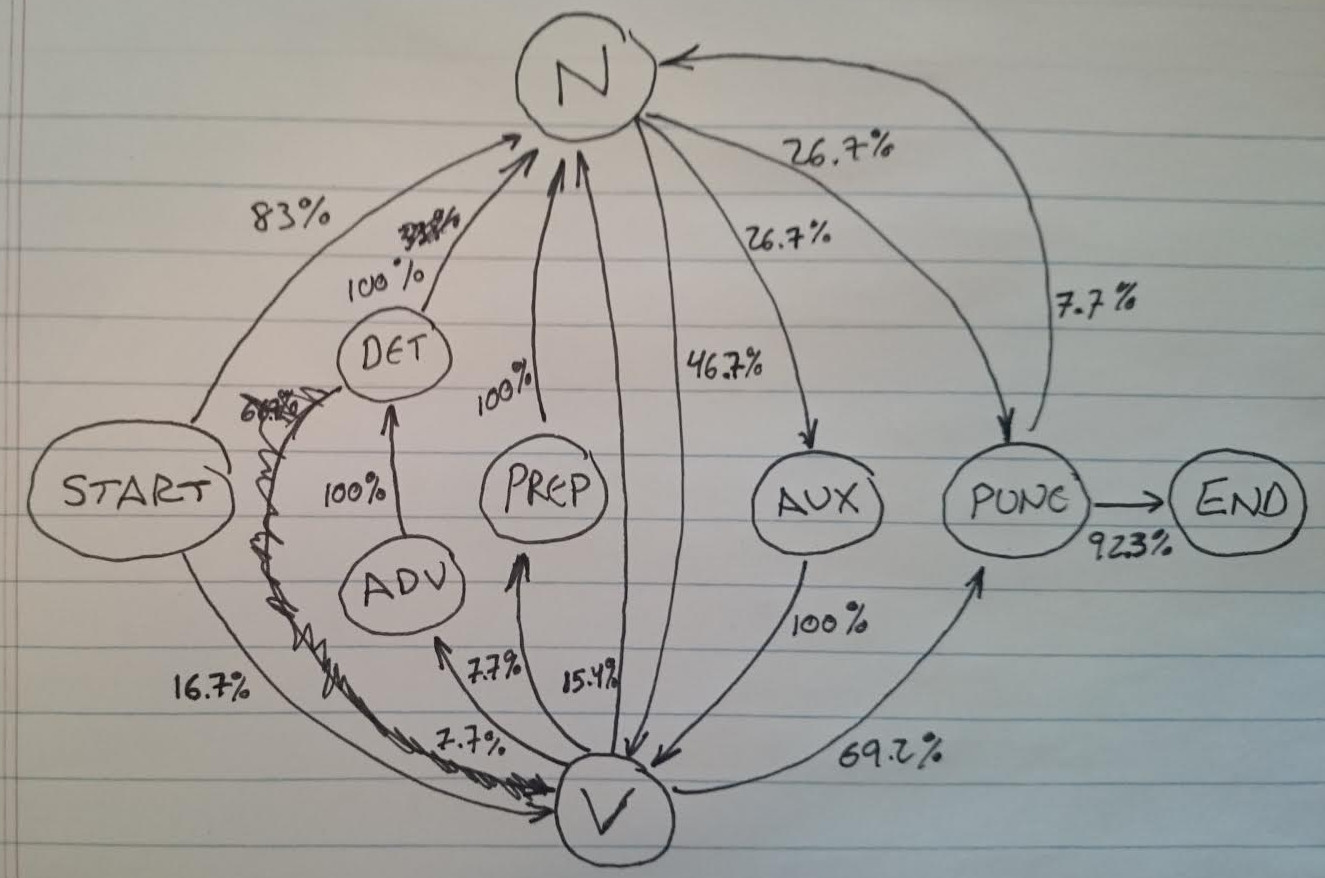
\includegraphics[width=\textwidth]{img/sample_hmm.jpg}
    \caption{Hand-drawn HMM model, trained on the sample dataset}
    \label{fig:sampleHmm}
\end{figure*}

\begin{figure*}
    \centering
    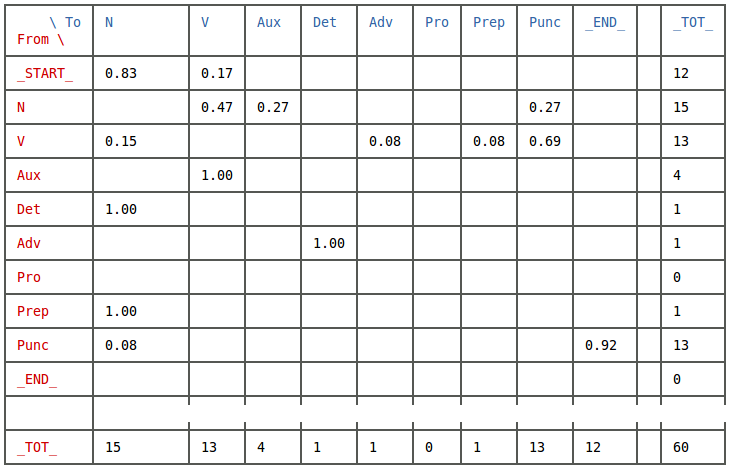
\includegraphics[width=150mm]{img/sample_transitions.png}
    \caption{Transition probabilities for sample dataset}
    \label{fig:sampleHmm_trans}
\end{figure*}

\clearpage
%
%\begin{figure*}
%    \centering
%    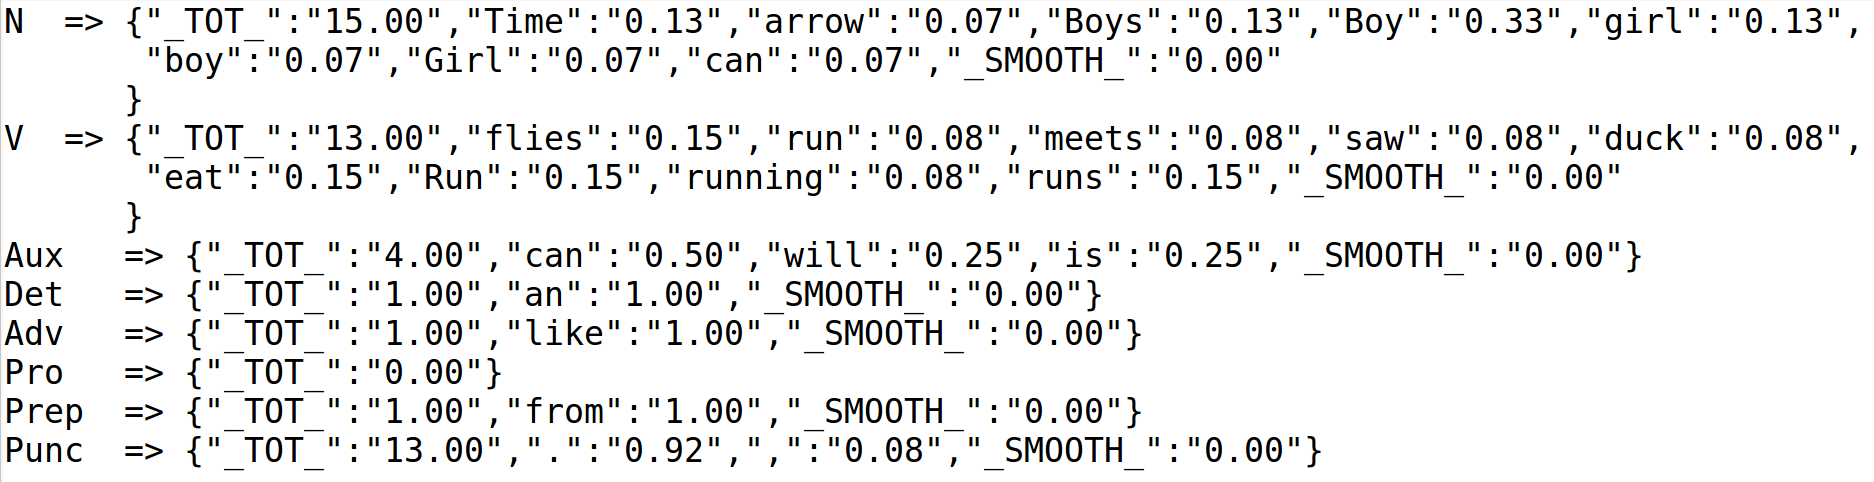
\includegraphics[width=150mm]{img/sample_outputs.png}
%    \caption{Output probabilities by tag for sample dataset}
%    \label{fig:sampleHmm_out}
%\end{figure*}


\begin{figure}
    \centering
    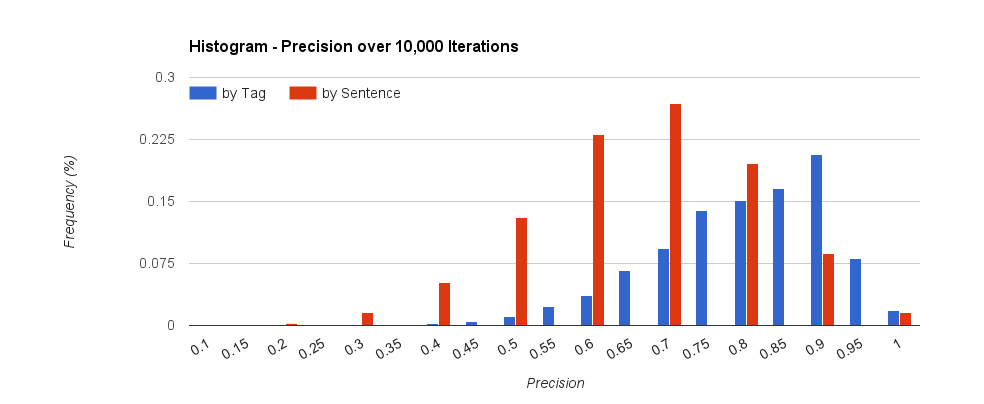
\includegraphics[width=\textwidth]{img/histogram_pcnt.png}
    \caption{A histogram of the precisions found over 10,000 iterations of the full dataset.}
    \label{fig:hist_freqs}
\end{figure}



\subsection{Full Dataset (Tasks 2-3)}
In analyzing the full dataset, only the labeled file was used (containing 108 tagged sentences).
The data was then partitioned into 90\% training and 10\% testing data.  After a sample run
with 10,000 iterations, the a mean tag precision of 80\% was found, shown in more detail in Table 2.

\begin{table}[h]
\begin{center}
\begin{tabular}{|l|l l|}
\hline \bf Precision  & \bf by Sentence & \bf by Tag \\ \hline
\bf Min  & 0.10 & 0.20 \\
\bf Mean & \bf 0.67 & \bf 0.80 \\
\bf Max  & 1.00 & 1.00 \\
\hline
\end{tabular}
\end{center}
\caption{\label{results} Results after 10,000 iterations on the full dataset. \\
Here, we show the precision both by sentence as well as by tag.}
\end{table}

Find a histogram of all results in Figure 4, effectively showing all possible precision for the
given partitioning ratio.



\section{Conclusion}
The Hidden Markov Model approach to modeling and applying sentence tagging is nearly trivial
to implement, while providing an apparently good precision on a small dataset of roughly
100 sentences.

While no significant challenges were found, the problem of how to appropriately smooth the
trained probabilites was not robustly dealt with.  This would be an area to apply
more effort into improving this HMM implementation.

\end{document}
